\documentclass[12pt,letterpaper]{article} % set main text size and page size
% \documentclass[10pt,a4paper]{article}
\usepackage[top=0.4in,bottom=0.4in,left=0.5in,right=0.5in]{geometry} % set page margins
\usepackage{charter} % select font (comment out lines to use Computer Modern)
\usepackage{graphicx} % Required for inserting images

% font and input encoding
\usepackage[T1]{fontenc}
\usepackage[utf8]{inputenc}
\usepackage{enumitem} % enable lists for bullet points: itemize and \item
\usepackage[hidelinks]{hyperref} % format hyperlinks
\usepackage{titlesec} % enable section title customization

% disable text justification
\raggedright

% disable page numbering
\pagestyle{empty}

% ensure that the PDF output will be all unicode and machine-readable
\input{glyphtounicode}
\pdfgentounicode=1

% format section headings: bolding, size, white space above/below
\titleformat{\section}{\bfseries\large}{}{0pt}{}[\vspace{1pt}\titlerule\vspace{-6.5pt}]

% format bullet points: size, white space above/below, white space between bullets
\renewcommand\labelitemi{$\vcenter{\hbox{\small$\bullet$}}$}
\setlist[itemize]{itemsep=-2pt, leftmargin=25pt}

%%%%%%%% resume starts here %%%%%%%%%
\begin{document}

\hfill{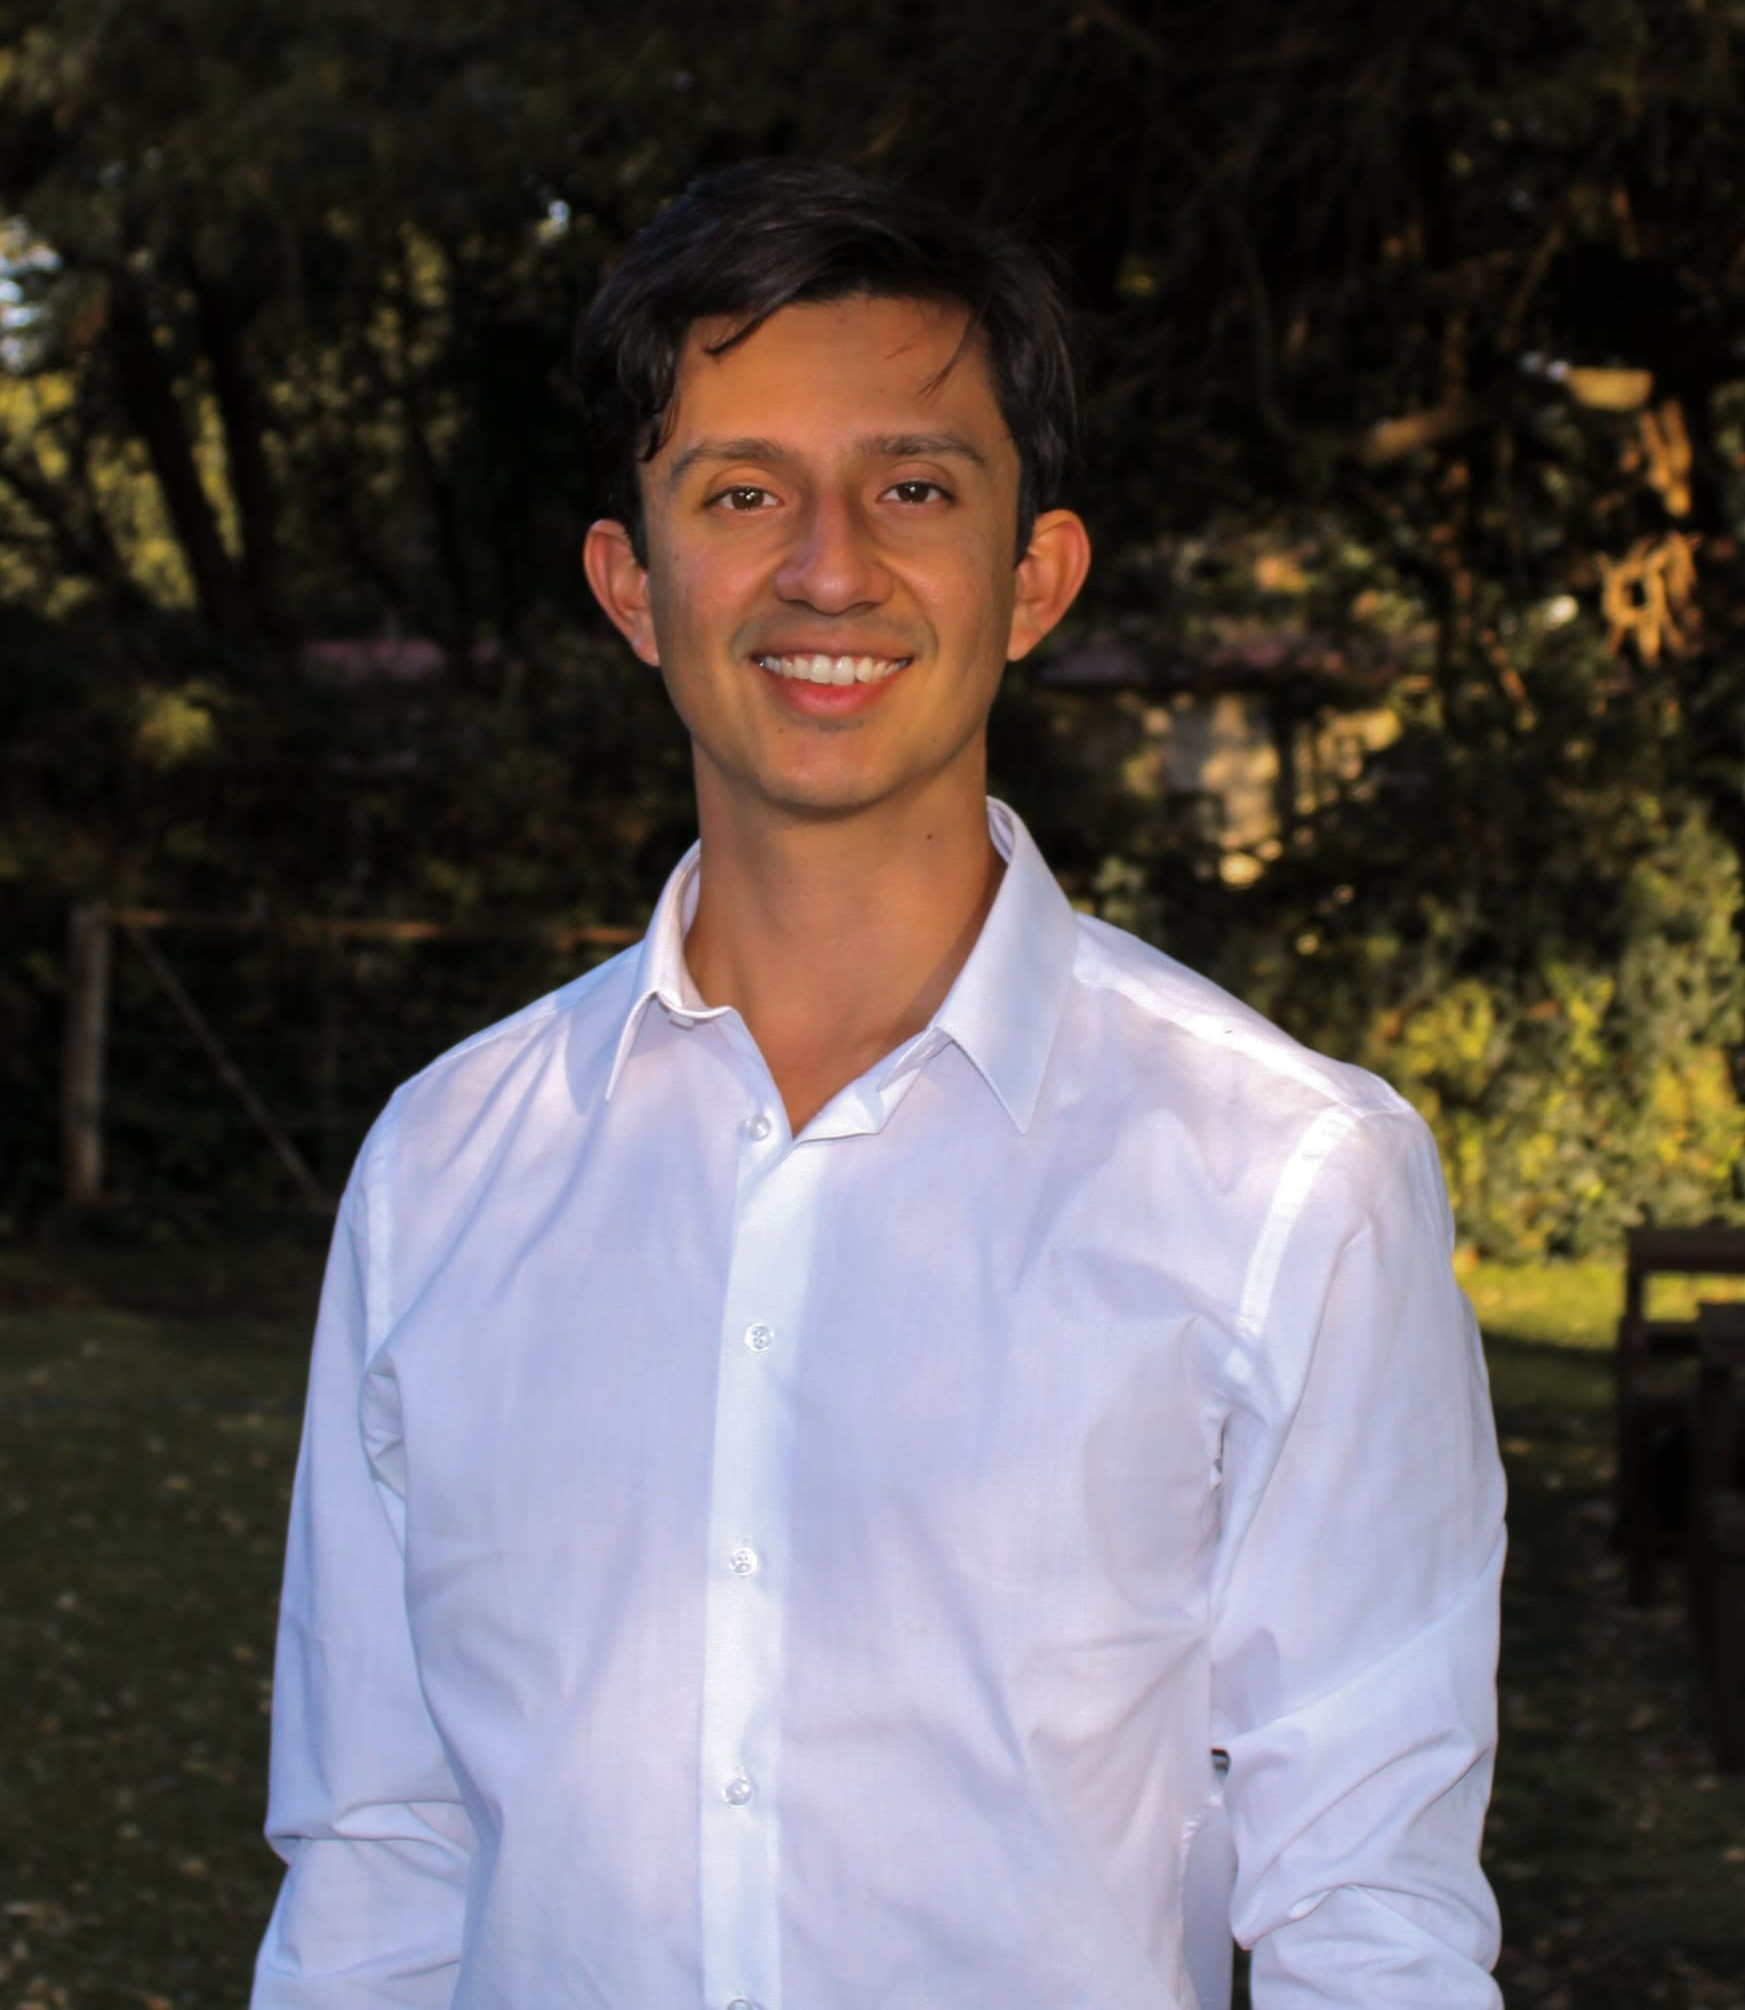
\includegraphics[width = 0.2\textwidth]{Headshot.jpg}}

\vspace{-120pt}
% name
\textbf{\large Richard D. Leyton-Romero} \\

\vspace{5pt} %spacing

% contact information

% 01-May-1996 \\
% richieleytongt@outlook.com \\
% \href{https://www.linkedin.com/in/richieleytongt/}{linkedin.com/in/richieleytongt} \\
% \href{https://github.com/richieleytongt}{github.com/richieleytongt} \\
% English + Español \\
% USA + Colombian dual national \\
% Johannesburg, South Africa 

\begin{tabular}{l l}
    \textbf{Date of Birth:} & 01-May-1996 \\
    \textbf{Email:} & richieleytongt@outlook.com \\
    \textbf{LinkedIn:} & \href{https://www.linkedin.com/in/richieleytongt/}{linkedin.com/in/richieleytongt} \\
    \textbf{GitHub:} & \href{https://github.com/richieleytongt}{github.com/richieleytongt} \\
    \textbf{Languages:} & English + Español \\
    \textbf{Nationality:} & USA + Colombian dual national \\
    \textbf{Location:} & Johannesburg, South Africa \\
    \end{tabular}

\vspace{-10pt} %spacing

%%%%%%% education section %%%%%%%
\section*{Education}

\textbf{\href{https://www.wits.ac.za/eie/}{University of the Witwatersrand}} -- PhD Electrical Engineering \hfill 2026 \\
\vspace{-15pt}
\begin{itemize}[itemsep=-4pt]
    \item \textbf{Research Focus:} Applied Optimal Control
    \item \textbf{Supervisor:} \href{https://www.nrf.ac.za/about-us/nrf-awards/2022-2/a-rated-researchers-2022/professor-david-j-n-limebeer/}{Professor David J.N. Limebeer}
    \item \textbf{Thesis:} The Usage of Optimal Control for Motorsport Performance Development
\end{itemize}

\vspace{-5pt}
\textbf{\href{https://www.brookes.ac.uk/courses/postgraduate/motorsport-engineering-msc}{Oxford Brookes University}} -- MSc Motorsport Engineering \hfill 2023 \\
\vspace{-9pt}
\begin{itemize}[itemsep =-4pt]
    \item \textbf{Dissertation:} The Effects of Race Vehicle Setup on Lap-by-Lap Tire Warm-Up Response
\end{itemize}

\vspace{-5pt}
\textbf{\href{https://www.usf.edu/engineering/me/}{University of South Florida}} -- BSME Mechanical Engineering \hfill 2020 \\
\vspace{-9pt}
\begin{itemize}[itemsep = -4pt]
    \item \textbf{Minor Degree:} Entrepreneurship
    \item \textbf{Senior Design:} Mazda BP4W Camshaft Design
\end{itemize}

\vspace{-25pt} %spacing

%%%%%%% experience section %%%%%%%

\section*{Experience}
\textbf{Owner/Operator,} Tampa Dynamics LLC -- Tampa, Florida \hfill 2019 -- 2023 \\
\vspace{3pt}
\textit{Provided race engineering support to motorsport organizations such as Pirelli Motorsport, Ian Lacy Racing, Ferrari of North America, Riley Technologies, and Multimatic Motorsports.}
\vspace{-5pt}
\begin{itemize}
  \item Optimized vehicle setups by assessing car and driver stability characteristics, leading to increased driver confidence.
  \item Leveraged driver-in-the-loop simulation to pinpoint location-specific performance and stability issues, ensuring thorough preparation before arrival to an event.
  \item Evaluated and optimized tire usage during track events by monitoring thermal activity and wear ensuring maximum vehicle performance.
\end{itemize}

\textbf{Mechanical Engineer,} \href{https://www.compcams.com/}{Comp Cams} -- Memphis, TN \hfill 2019 \\
\vspace{-9pt}
\begin{itemize}
%   \item Solved a common Chrysler engine failure by identifying critical point of defect and redesigning hydraulic valvetrain lifter to allow for free flow of oil.
  \item Tuned control parameters for vintage Chevrolet engine retrofitted with modern electronic fuel injection by monitoring and adjusting air:fuel ratios and spark timing.
  \item Provided powertrain consulting for race teams across various motorsport categories from professional drag racing to boat racing.
\end{itemize}

\vspace{-20pt} %spacing

%%%%%%% publications section %%%%%%%

\section*{Publications}

Limebeer, D. J. N., Leyton Romero, R. D., and Massaro, M. (2025). An optimal control approach to the generation of yaw-moment diagrams. \textit{Vehicle System Dynamics}, 1–25. \href{https://doi.org/10.1080/00423114.2025.2471344}{doi.org/10.1080/00423114.2025.2471344}

\vspace{-10pt} %spacing

%%%%%%% skills section %%%%%%%
\section*{Skills}
\textbf{Programming and Computation} MATLAB, Python, Maple, Mathematica, \\
\textbf{Mechanical Design and Simulation:} SOLIDWORKS (certified), CATIA V5, LS-DYNA, STAR-CCM+ \\
\textbf{Motorsport Data Visualization:} MoTeC i2, Cosworth Pi, WinTax4 \\



%%%%%% resume ends here %%%%%%%

\end{document}